\documentclass[11pt]{article}
%Gummi|061|=)
\usepackage{hyperref}
\usepackage{url}
\usepackage[spanish]{babel}
\usepackage[utf8]{inputenc}
\usepackage{pdfpages}
\title{\textbf{Práctica sobre Arquitecturas: LogProcessor}}
\author{Israel Pavón Maculet - Sergio Arroutbi Braojos}
\selectlanguage{spanish}
\date{\today}
\usepackage[bottom=14em]{geometry}
\usepackage{amsmath}
\usepackage{mathtools}
\usepackage{float}
\usepackage{pdflscape}
\usepackage{geometry}

\begin{document}

\restylefloat{table}
\restylefloat{figure}

\hypersetup
{   
pdfborder={0 0 0}
}
   
\maketitle

\pagebreak

\tableofcontents

\pagebreak

\section{Introducción}
En esta práctica se pretende realizar el diseño arquitectónico de una solución de recolección de logs. En particular, se trata de diseñar un sistema que a partir de dos tipos de logs, logs de sistema y logs de aplicación, con sus respectivos formatos, distintos entre sí, se genere un único tipo de log que pueda ser analizado posteriormente.

A priori, se generarán dos tipos de logs por parte de las aplicaciones y sistemas ya existentes. Posteriormente, dichos logs se recibirán por un sistema dedicado que los tratará de procesar a un único formato intermedio standard. Finalmente, habrá una etapa de análisis que permitirá realizar ciertas acciones en función del contenido del log en formato standard.

Este documento no pretende describir la práctica, ya que su enunciado puede consultarse en el siguiente link:

\url{https://drive.google.com/folderview?id=0BwwK87eKaiN_dlgzZ1pEamRwM1k&usp=sharing_eid&tid=0B2GOgs_VnHZuflF3bXJnUmZkTHdxbFJPNGNmZjE3SHhYWDljUC10eC12W}

Se prentende más bien enunciar aquellas decisiones de diseño arquitectural llevadas a cabo, teniendo en cuenta el tipo de aplicación que se pide, el patrón o conjunto de patrones arquitectónicos que se pueden aplicar para obtener llegar a una solución y las iteraciones realizadas hasta afinar la arquitectura seleccionada.

\pagebreak

\section{Justificación sobre la elección de la arquitectura}

\subsection{Elección del patrón: Pipes \& Filters}
En una primera instancia, la decisión que se ha llevado opta por la elección del patrón de arquitectura “Pipes \& Filters”, ya que el patrón está orientado a proporcionar una estructura que permite organizar la aplicación orientada al procesamiento de un flujo de datos.

En este caso, el flujo de datos son los logs que recibe la aplicación y que requieren una serie de procesados y acciones. En este caso, las diferentes acciones y etapas que realiza la aplicación sobre los logs pueden encajar bien en el concepto de filtro, y el modo de ir transportando los logs en sus diferentes etapas de procesado y análisis, serían los pipes.

\subsubsection{Fuerzas}

Las fuerzas que han hecho que la arquitectura por la que se opta por empezar con un planteamiento orientado a este patrón de Ps\&Fs, son las siguientes:

\begin{itemize}
\item{El hecho de tener como requisito una serie de etapas de procesamiento, que deben de ser cambiadas de forma “fácil” y dinámica, se considera que encaja con las fuerzas especificadas en la descripción del patrón.}
\item{Por otro lado, se considera que al dividir en detalle las acciones a realizar sobre los logs, salen etapas pequeñas que se podrán reutilizar.}
\item{Parece que el heco de tener distintas fuentes de datos (distintas aplicaciones/hosts que envían logs al sistema), es otro de los puntos que considera el patrón como fuera para su uso.}
\item{Por último, también se observa en el análisis del problema que hay etapas que consideramos que se pueden paralelizar, por ejemplo, los análisis de los logs pueden ser paralelos, con lo que tendríamos otra razón que encaja con las fuerzas del patrón.}
\end{itemize}

\subsubsection{Consecuencias}

La eliminación del fichero de standarLogs y su conversión en una cola de publicación permite ahorrar el uso de ficheros intermedios y proporcionar la posibilidad de paralelizar la fase de análisis.

Este tipo de patrón permite, además, cambiar los filtros de forma o sencilla, o incluso en runtime, algo que es un requisito del sistema. Al usar este patrón, existirá la posibilidad de combinar y reutilizar los filtros que se usen para procesar los logs, lo que se considera muy interesante a priori.

Aunque no es exclusivo de este patrón, el hecho de tener filtros independientes permite poder afrontar el desarrollo de forma paralela por diferentes personas, con una integración más sencilla de las diferentes partes.

\subsubsection{Responsabilidades}

Una de las desventajas que tiene este patrón será el compartir el estado de los diferentes filtros. En este caso, tras el estudio incial, no vemos la necesidad de que el estado necesite ser compartido. Por ejemplo, el hecho de que el procesador esté en el estado “analizando severidad”, no interfiere en el comportamiento del analizador.

Aunque hay filtros que no se ejecuten realmente en paralelo y sea necesario que un filtro tenga que procesar completamente los datos, en nuestro caso, no vemos una alternativa, ya que el analizador necesita un log estándar, así que si el procesado no lo ha llegado a generar, no tiene nada que analizar. Por tanto esta responsabilidad es asumible.

No obstante, en un primer análisis, hemos previsto la posibilidad de tener N procesos de análisis corriendo en paralelo, con lo que hay fases que sí se podrán paralelizar de manera real.

Si bien este patrón indica que la gestión de errores puede ser compleja, no hay requisitos específicos que impacten en esta desventaja.

\subsection{Elección del patrón: Pipes \& Filters + Broker}

Una vez analizadas las fuerzas, consecuencias y responsabilidades de utilizar el patrón Pipes\&Filters, se ha llegado a la conclusión que el uso en exclusiva de este patrón no permite atender la naturaleza del sistema.

El principal motivo de este hecho es la naturaleza distribuída del sistema. El patrón Pipes\&Filters es simplemente insuficiente para atender las comunicaciones que se tienen que prodcuir entre los distintos elementos del sistema propuesto.

Por un lado, existen "clientes" del sistema, que son los generadores de logs. Por otro lado, existe un componente de análsis y parseo de los logs que permite unificar el formato de los logs, de forma que se obtiene un formato común que diversos analizadores podrán analizar a posteriori. Finalmente, éstos analizadores se configurarán de forma que se podrán realizar diversas acciones de forma configurable, como, por ejemplo, la generación de ficheros según keywords.

Todo esto hace entrever que estamos ante un tipo de sistema distribuido, heterogéneo y con diversos componentes de distinta naturaleza que cooperan entre sí. Este es, sin duda, el contexto definido para el patrón arquitectural conocido como "Broker", un patrón que permite implementar aplicaciones monolíticas, potencialmente escalables, que permite definir un marco para la comunicación entre procesos así como una fácil integración de componentes adicionales en el sistema.

Por tanto, la arquitectura final elegida para el sistema es un híbrido entre Pipes\&Filters y Broker, en la que, existen tres componentes heterogéneos y distribuídos en el sistema (generadores de logs, procesador de logs y analizadores de logs estándard) que cooperan entre sí para proporcionar la funcionalidad final de forma distribuida. Esta comunicación se apoyará en el patrón Broker, de forma que cada uno de estos componentes sepa como comunicarse con aquellos otros componentes con los que necesita cooperar.

Además, dentro de uno de estos componentes, en concreto dentro del procesador de logs, se considera que aplica el patrón Pipes\&Filters, por los motivos detallados en el capítulo anterior.

\pagebreak

\section{Documentación: Modelo de 4+1 vistas}

En este apartado se detalla el modelo de 4+1 vistas. Este modelo, diseñado por Philippe Kruchten, permite mostrar distintos enfoques desde el punto de vista arquitectónico para la solución que se propone.

\begin{center}
 \begin{figure}[H]
 \begin{center}
   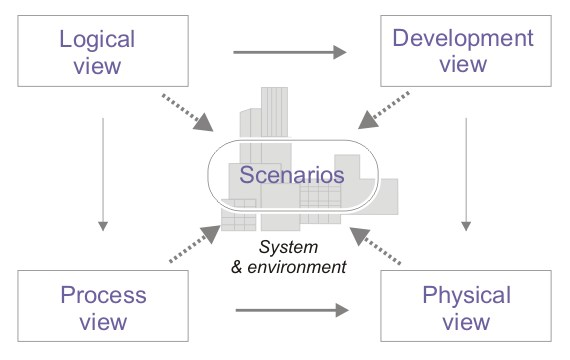
\includegraphics[width=10cm]{img/4+1view.jpg}
   \caption{4+1 Architectural View Model}
   \label{fig:4plus1views}
 \end{center}
 \end{figure}
\end{center}

A continuación se muestran las distintas vistas que propone este modelo para la solución propuesta.

\subsection{Vista Lógica}

En esta vista se debe incluir informacion que permita detallar la funcionalidad que el sistema proporciona de cara al usuario final. Para ello se deben incluir diagramas de clases, de comunicacion y/o de secuencia.

Para esta solución, el diagrama de clases que se propone se muestra a continuación:

\begin{center}
 \begin{figure}[H]
 \begin{center}
   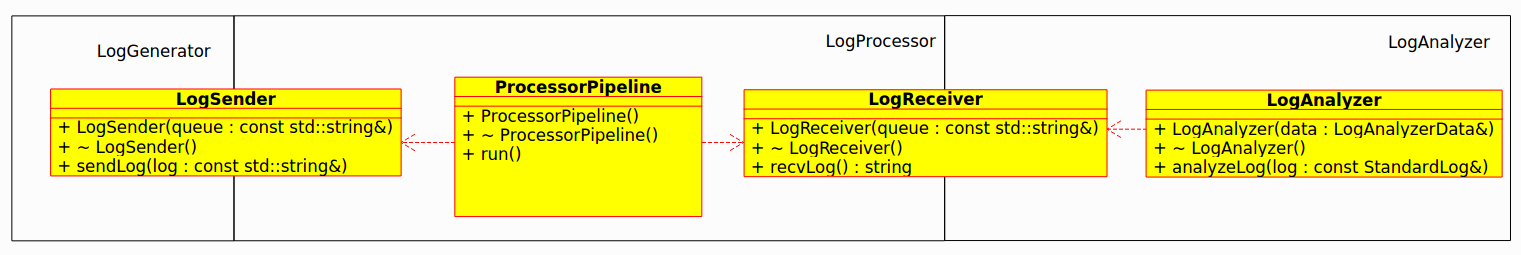
\includegraphics[width=15cm]{img/classes_summary01.png}
   \caption{Vista Lógica: Diagrama de clases}
   \label{fig:4plus1views}
 \end{center}
 \end{figure}
\end{center}

Cabe decir que la vista anterior simplemente muestra una vista reducida de las principales clases que se implementarán en la solución. Cada uno de los procesos propuestos se apoyarán en clases adicionales para realizar la funcionalidad deseada. Este mayor nivel de detalle se mostrará en la vista de implementación.

\subsection{Vista de Implementación}

Este tipo de vista recoge aquellos detalles que tienen que ver con la gestión del software, y más concretamente con cómo el sistema está compartimentado en distintos paquetes de software que permiten llegar a la solución final. Normalmente, la forma en la que se detalla este tipo de vista es a través de diagramas de componentes y/o diagramas de paquetes que permitan mostrar aquellos artefactos que tiene el software y cómo se agrupan entre sí.

En el caso del procesador de logs, esta vista viene representada por los diagramas que se muestran a continuación:

\begin{center}
 \begin{figure}[H]
 \begin{center}
   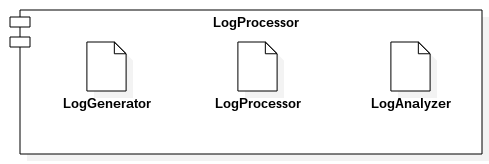
\includegraphics[width=15cm]{img/implementation_view00.png}
   \caption{Vista de Implementación: Artefactos}
   \label{fig:4plus1views}
 \end{center}
 \end{figure}
\end{center}

Como puede observarse, el sistema consta de tres ejecutables que permiten enviar, procesar y analizar logs respectivamente. Así, cada uno de los artefactos a su vez están compuestos por distintas clases que les permiten llevar a cabo la funcionalidad siguiendo los principios de diseño SOLID. Se describe el detalle de implementación de cada paquete a continuación:

\newgeometry{top=0cm,left=0cm,bottom=0.3cm}
\begin{landscape}
\begin{center}
 \begin{figure}[H]
 \begin{center}
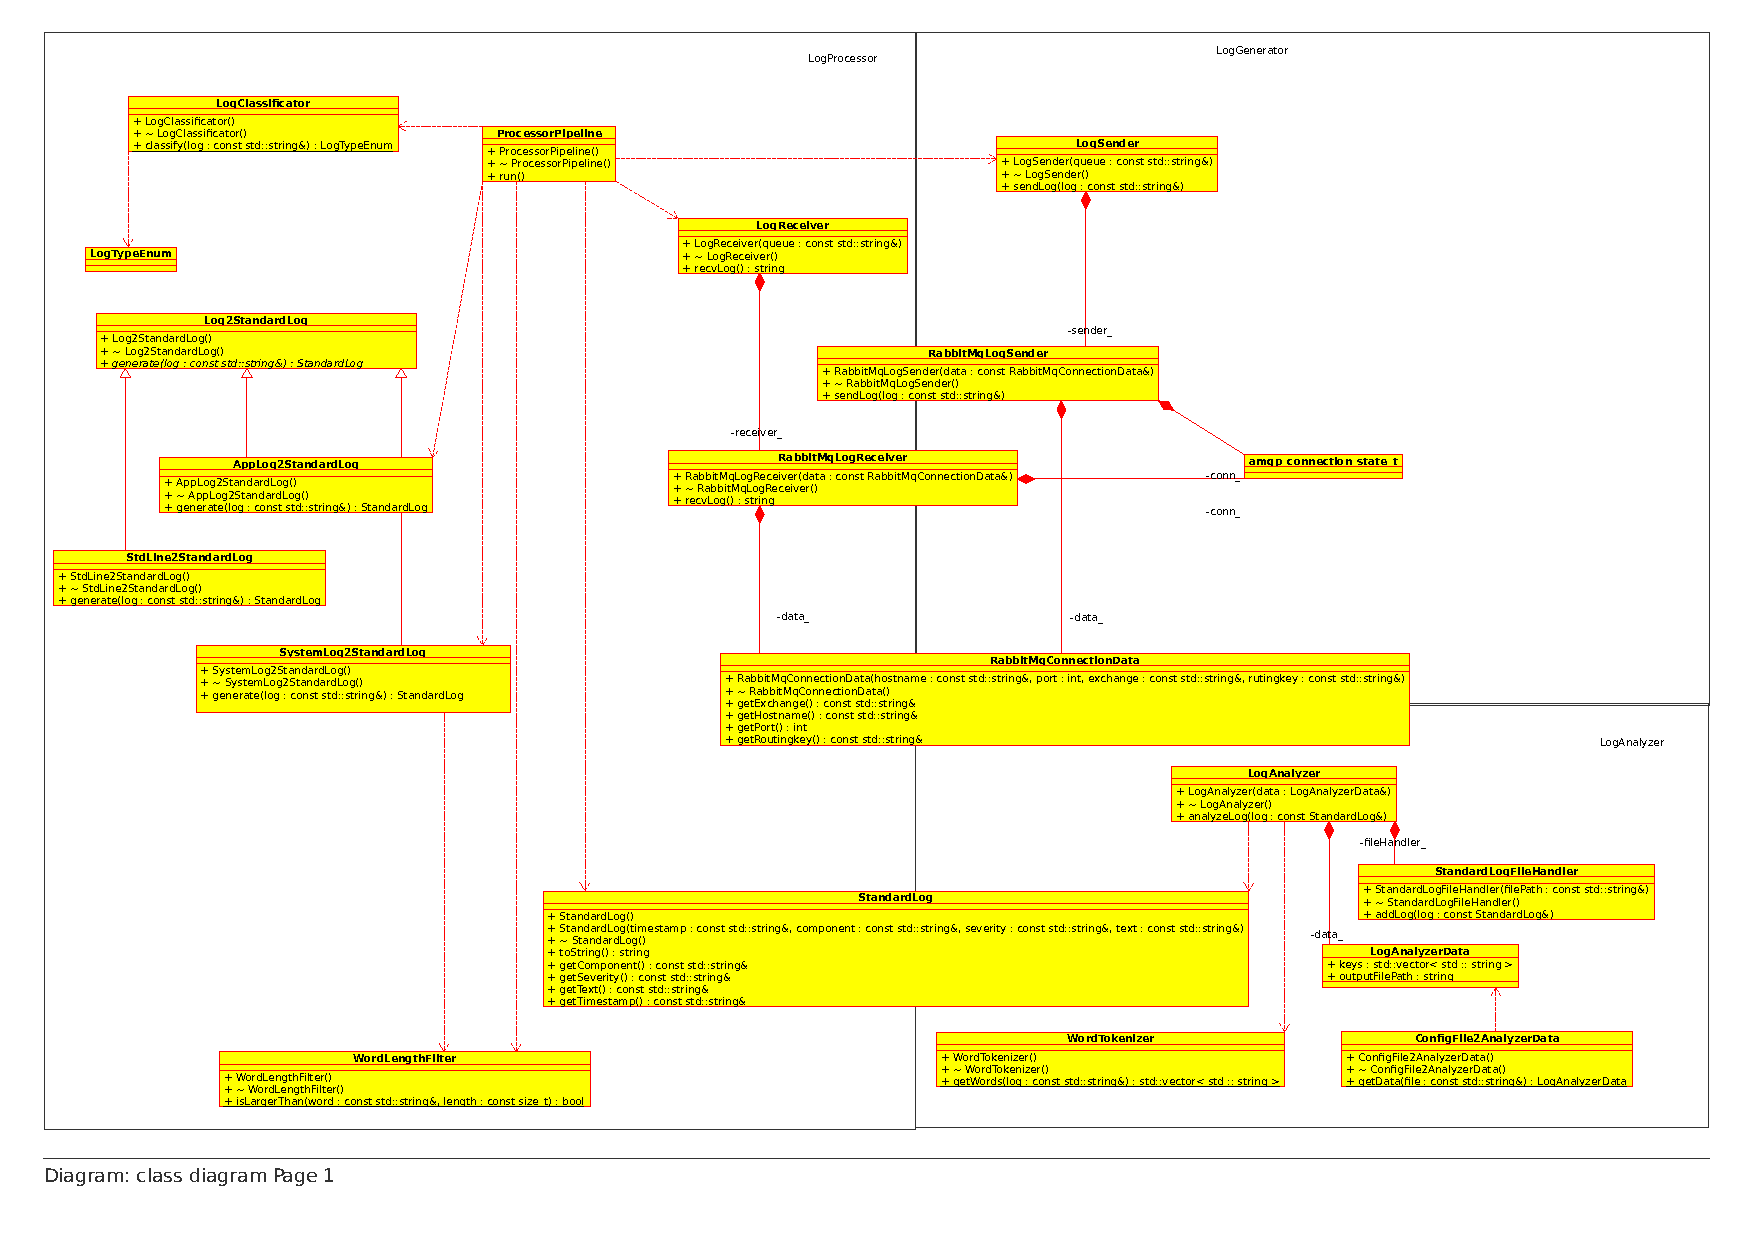
\includegraphics[scale=0.85]{classes01.pdf}
   \label{fig:classes_per_component}
 \end{center}
 \end{figure}
\end{center}
\end{landscape}
\restoregeometry

\subsection{Vista de Procesos}
Esta vista debe mostrar aquellos procesos que existen en el sistema en tiempo de ejecución, cómo se comunican entre sí y qué mensajes intercambian. Los diagramas de actividad o de secuencia permiten realizar una descripción de este tipo de sistemas. A continuación, se muestra el diagrama de secuencia elegido para esta solución:

\begin{center}
 \begin{figure}[H]
 \begin{center}
   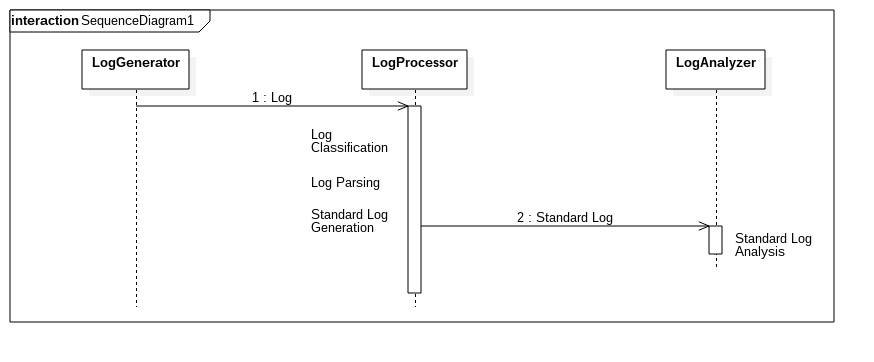
\includegraphics[width=16cm]{img/process_view00.png}
   \caption{Vista de Procesos}
   \label{fig:4plus1views}
 \end{center}
 \end{figure}
\end{center}

\subsection{Vista Física (o de despliegue)}
En esta vista se detalla el despliegue de los distintos artefactos en distintas máquinas físicas. Un diagrama de despliegue permite ver cómo se reparten los distintos artefactos identificados en la vista de implementación.

De esta forma, esta vista pretende documentar aquellas máquinas existentes en el sistema, los artefactos existentes en cada una así como detalles de comunicaciones entre las máquinas.

Cualquier tipo de información interesante para el personal encargado de despliegue debe aparecer, de forma que los operarios de despliegue cuenten con diversos detalles que luego pueden resultar útiles a la hora de configurar elementos de red, seguridad, etc.

Así, para esta solución se propone el siguiente diagrama de despliegue:

\newgeometry{top=0cm,left=3cm,bottom=0.3cm}
\begin{landscape}
\begin{center}
 \begin{figure}[H]
 \begin{center}
   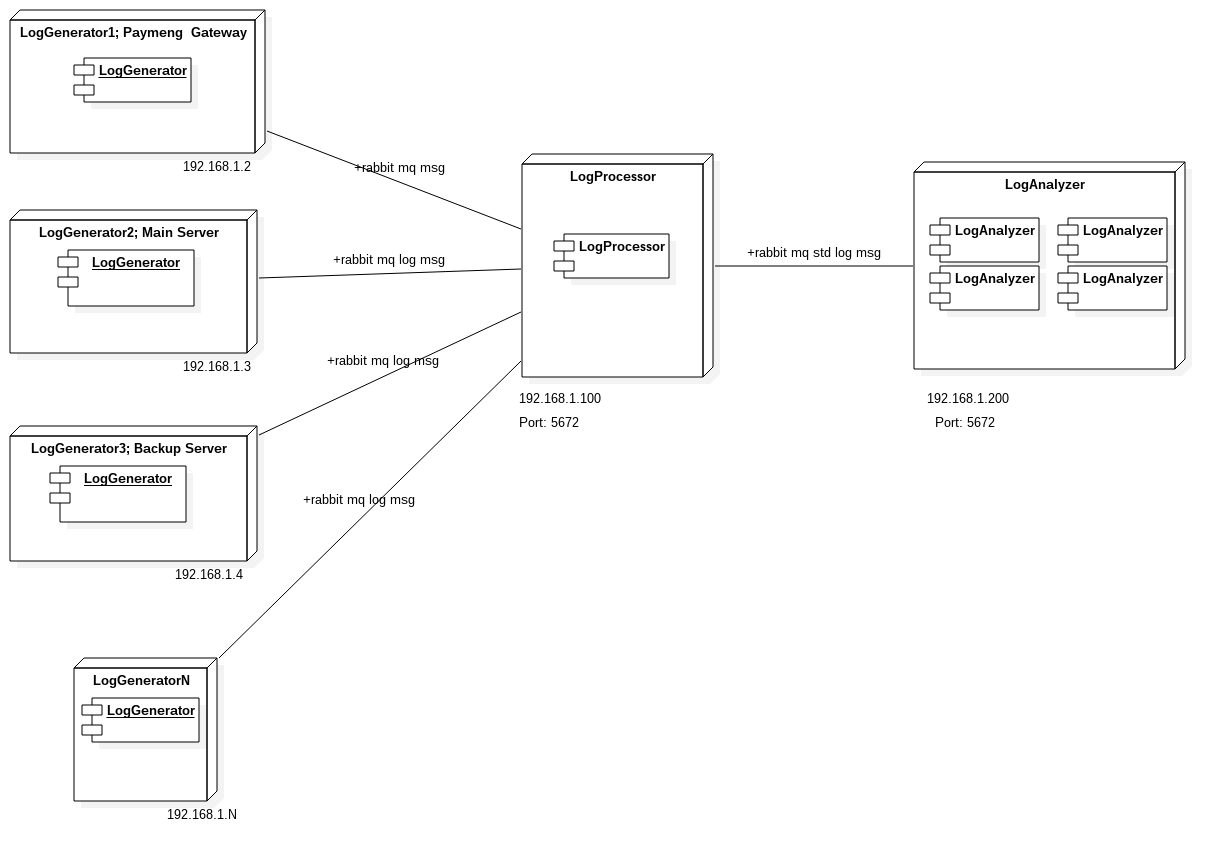
\includegraphics[width=20.5cm]{img/physical_view00.png}
   \caption{Vista de Despliegue}
   \label{fig:4plus1views}
 \end{center}
 \end{figure}
\end{center}
\end{landscape}
\restoregeometry

\subsection{Vista de Escenario}

\pagebreak

\section{Implementación}

\end{document}
